\documentclass[12pt,a4paper]{scrartcl}

%========================================================================================
%SPRACHE

\usepackage[ngerman]{babel} 
\usepackage[T1]{fontenc} 				% richtige Silbentrennung
\usepackage[utf8]{inputenc}

% schicke Typographie
\usepackage{charter}
\usepackage[stretch=10,shrink=10]{microtype} 
\usepackage[expert]{mathdesign}
%========================================================================================
%DARSTELLUNG

\usepackage[small,compact]{titlesec} 		% Verkleinerung von Section-Ueberschriften
\usepackage{graphicx}				  	% Einbinden von Graphiken .ps, .pdf, .png

\usepackage{amsmath}					% mathematische Symbole
\setlength{\parindent}{0pt}				% Zeile nach Absatz einruecken 1pt oder nicht 0pt.

\usepackage{float} % alles möglichen Sachen mit [h] an die richtige Stelle zwingen

\titleformat{\section}[hang]{
    \usefont{T1}{qhv}{b}{n}\selectfont} % "qhv" - TeX Gyre Heros, "b" - bold
    {} 
    {0em}
    {\hspace{-0.8em}\Large \hspace{0.6em}}

\titleformat{\subsection}[hang]{
    \usefont{T1}{qhv}{b}{n}\selectfont} % "qhv" - TeX Gyre Heros, "b" - bold
    {} 
    {0em}
    {\hspace{-0.7em}\large \hspace{0.6em}}
    
\titleformat{\subsubsection}[hang]{
    \usefont{T1}{qhv}{b}{n}\selectfont} % "qhv" - TeX Gyre Heros, "b" - bold
    {} 
    {0em}
    {\hspace{-0.6em}\normalsize \hspace{0.6em}}

%========================================================================================
%FARBEN

\usepackage[usenames,dvipsnames]{color}	

									%Apricot 	Aquamarine 	Bittersweet 	Black
									%Blue 	BlueGreen 	BlueViolet 	BrickRed
									%Brown 	BurntOrange 	CadetBlue 	CarnationPink
									%Cerulean 	CornflowerBlue 	Cyan 	Dandelion
									%DarkOrchid 	Emerald 	ForestGreen 	Fuchsia
									%Goldenrod 	Gray 	Green 	GreenYellow
									%JungleGreen 	Lavender 	LimeGreen 	Magenta
									%Mahogany 	Maroon 	Melon 	MidnightBlue
									%Mulberry 	NavyBlue 	OliveGreen 	Orange
									%OrangeRed 	Orchid 	Peach 	Periwinkle
									%PineGreen 	Plum 	ProcessBlue 	Purple
									%RawSienna 	Red 	RedOrange 	RedViolet
									%Rhodamine 	RoyalBlue 	RoyalPurple 	RubineRed
									%Salmon 	SeaGreen 	Sepia 	SkyBlue
									%SpringGreen 	Tan 	TealBlue 	Thistle
									%Turquoise 	Violet 	VioletRed 	White
									%WildStrawberry 	Yellow 	YellowGreen 	YellowOrange
									
									% verwenden mit: 
									% \pagecolor{declared-color}
									% {\color{declared-color} text}
									% \colorbox{declared-color1}{\color{declared-color2} text}

									%========================================================================================
%Zur Einbindung von Programmiertexten mit:
				% \begin{lstlisting}
				%put your code here
				%\end{lstlisting}
				
\usepackage{listings}
\lstset{ %
language=matlab,                			% the language of the code
basicstyle=\ttfamily,       			% the size of the fonts that are used for the code
numbers=left,                   				% where to put the line-numbers
numberstyle=\tiny,      			% the size of the fonts that are used for the line-numbers
stepnumber=1,                   				% the step between two line-numbers. If it's 1, each line 
                                					% will be numbered
numbersep=5pt,                  			% how far the line-numbers are from the code
backgroundcolor=\color{white},  		% choose the background color. You must add \usepackage{color}
showspaces=false,               			% show spaces adding particular underscores
showstringspaces=false,        		 	% underline spaces within strings
showtabs=false,                 				% show tabs within strings adding particular underscores
frame=b,                   				% adds a frame around the code
tabsize=2,                      				% sets default tabsize to 2 spaces
captionpos=t,                   				% sets the caption-position to bottom
breaklines=true,                				% sets automatic line breaking
breakatwhitespace=false,        			% sets if automatic breaks should only happen at whitespace
%title=\lstname,                 				% show the filename of files included with \lstinputlisting;
                                					% also try caption instead of title
}
%========================================================================================

% geile captions!
\usepackage{caption}
\DeclareCaptionFont{white}{\color{white}}
\DeclareCaptionFormat{listing}{\colorbox{Gray}{\parbox{\textwidth}{#1#2#3}}}
\captionsetup[lstlisting]{format=listing,labelfont=white,textfont=white}

% links
\usepackage[]{hyperref}

\definecolor{darkblue}{rgb}{0,0,.5}
\hypersetup{pdftex=true, colorlinks=true, breaklinks=true, linkcolor=darkblue, menucolor=darkblue, pagecolor=darkblue, urlcolor=darkblue}

%LOAD FANCYHDR fuer Kopf- und Fusszeilen
\usepackage{fancyhdr}					% Paket laden	für einfache Handhabung von Kopf-und Fu{ß}zeile
\pagestyle{fancy}							
\fancyhf{}
\fancyhead[L]{\small{\textbf{Migration Seismischer Daten \\ Semesterabschlussarbeit}}}
\fancyhead[R]{\small{Sebastian Beyer und Denys Zhurovich \\ 7. April 2013}}
\fancyfoot[C]{\thepage} 			%Seitennummer



\usepackage{subfigure}

\addto\captionsngerman{
\renewcommand{\figurename}{Abb.}
\renewcommand{\tablename}{Tab.}
}

\usepackage{booktabs}




\begin{document}


\section*{Migration Seismischer Daten}

\subsection*{Aufgabe 2}


Nun gilt es, synthetische Seismogramme zu migrieren.

Dazu schreiben wir ein Modul in \textit{Pyhton}, in welchem wir die benötigten Prozeduren als Funktionen implementieren.

Dieses Modul laden wir im interaktiven Pyhton-Interpreter:

\begin{verbatim}
>>> import kirchhoffmigration as k
\end{verbatim}

Nun können wir die Daten darstellen (Abb. \ref{unprocessed}):

\begin{verbatim}
>>> k.PlotImg(k.data,'unprocessed')
\end{verbatim}

\begin{figure}[htb]
\centering
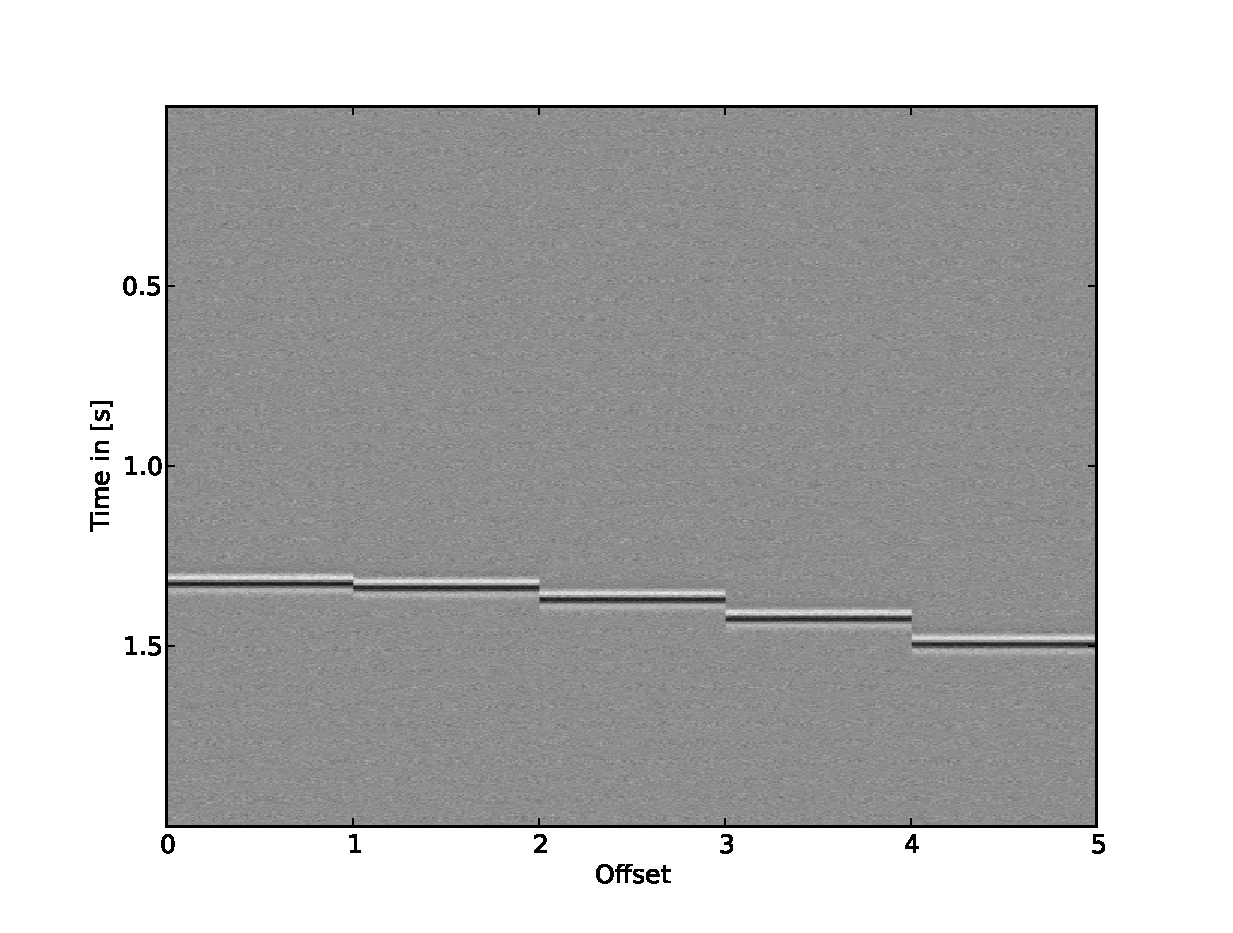
\includegraphics[width=1\textwidth]{unprocessed}
\caption{Unprozessierte Daten}
\label{unprocessed}
\end{figure}

\subsubsection*{a. - Frequenzgehalt der Daten}

Um den Frequenzgehalt der Daten abschätzen zu können, verwenden wir die \textit{fast Fourrier Transformation} aus dem \textit{SciPy}-Modul\footnote{\url{http://www.scipy.org}}.

\begin{verbatim}
>>> k.PlotSpectrum(1)
\end{verbatim}

In Abbildung \ref{spectrum} ist zu erkennen, dass die Hauptfrequenz des Signals bei ca. 25 Hertz liegt. 
Damit liegt sie deutlich unter der Nyquist Frequenz von 250 Hertz. Die Abtastfrequenz hätte also noch niedriger gewählt werden können, um Datenvolumen und damit Speicherplatz und Rechenzeit zu sparen.

\begin{figure}[htb]
\centering
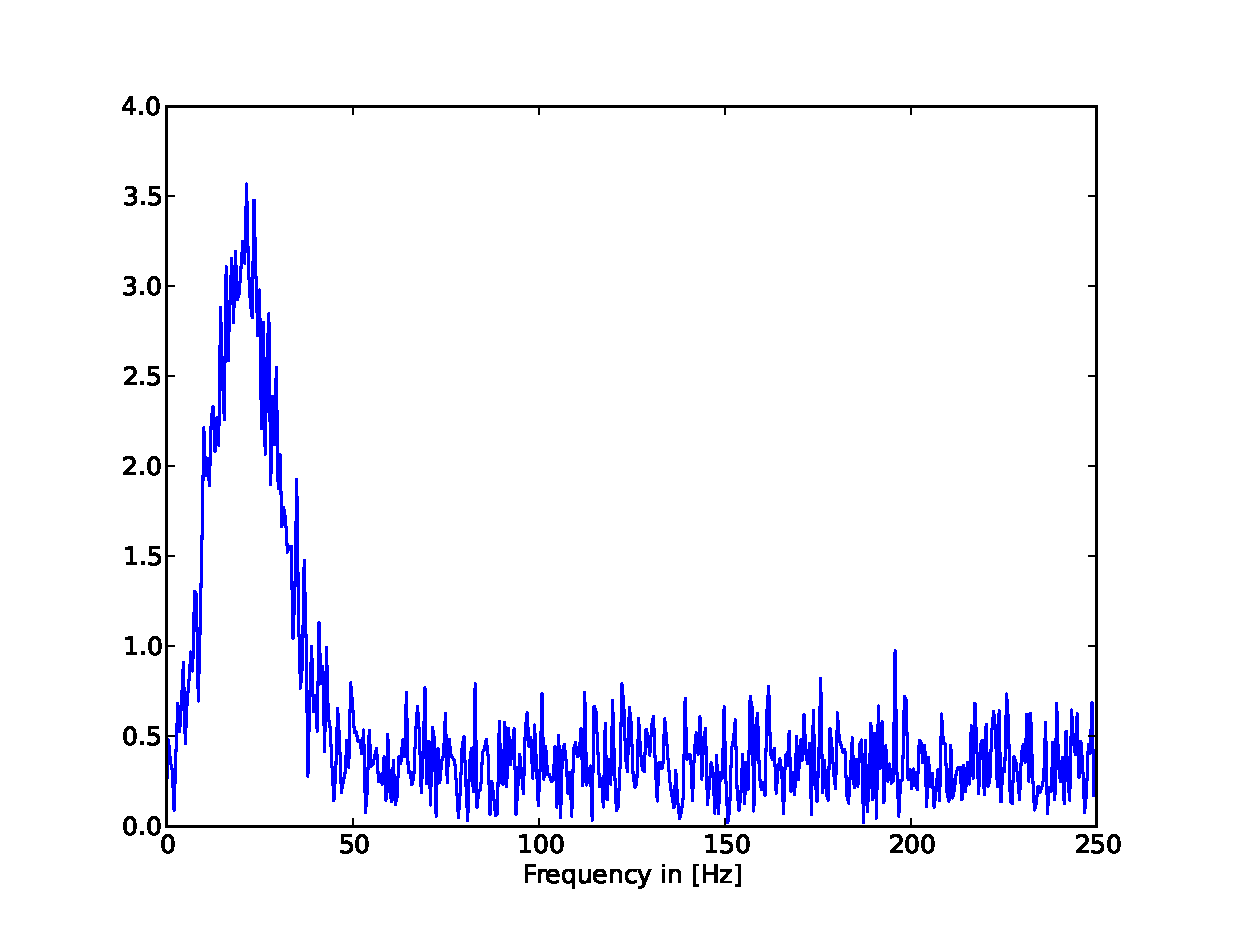
\includegraphics[width=1\textwidth]{spectrum}
\caption{Spektrum der 2. Spur der Originaldaten}
\label{spectrum}
\end{figure}



\subsubsection*{b. - Migrationsverfahren}

Da die Daten als \textit{Constant Offset Gather} vorliegen, bietet sich eine \textit{Kirchhoff Inversion} an. 

Hierbei diskretisieren wir zunächst den Untergrund und summieren dann für jeden Untergrundpunkt die dazugehörigen (auf seiner virtuellen Diffraktionshyperbel liegenden) Reflektivitäten aus den Daten auf. 

Der Vorteil dieser Methode ist, dass wir sowohl das Abbild als auch die Reflexionsamplituden rekonstruieren können (\textit{True Amplitude Migration}. Dadurch lassen sich möglicherweise Rückschlüsse auf die Schereigenschaften (und damit Porosität und Permeabilität) des Materials ziehen.


\begin{figure}[htb]
\centering
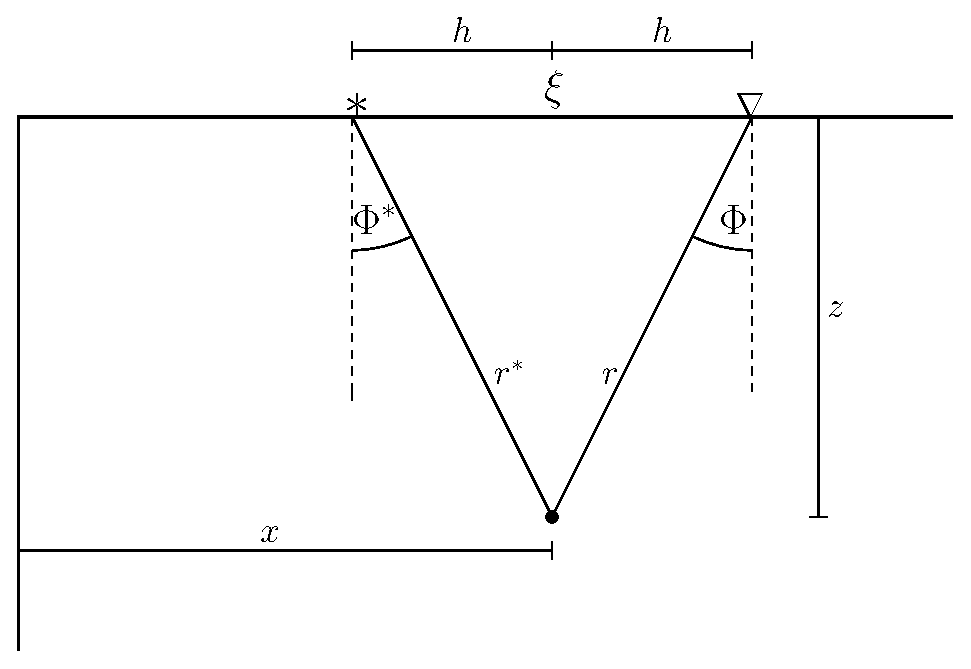
\includegraphics[width=0.8\textwidth]{kirchhoffgeometrie}
\caption{Geometrie der Kirchhoff Inversion}
\label{kirchhoffgeometrie}
\end{figure}


Aus dem Skript wissen wir:

\begin{equation}
	R(x,z) = \int\limits_{-\infty}^{\infty} 
		d\xi \quad u_F(\xi,z=0,\frac{r^*+r }{v})
		\quad \omega_{CO} \frac{1}{\sqrt{2 \pi}}
\end{equation}
mit
\begin{equation}
	\omega_{CO} = \frac{1}{v} \quad ( \cos \Phi \sqrt{\frac{r^*}{r}} + 
		\cos \Phi^* \sqrt{\frac{r}{r^*}})
\end{equation}




Aus geometrischen Überlegungen in Abbildung \ref{kirchhoffgeometrie} erhalten wir:

\begin{eqnarray}
	r^* = \sqrt{ (x-(\xi - h))^2 + z^2 }  \\
	r = \sqrt{ (x-(\xi + h))^2 + z^2 }
\end{eqnarray}

und

\begin{eqnarray}
	\Phi^* = \arccos( \frac{z}{r^*} )	\\
	\Phi = \arccos ( \frac{z}{r} )
\end{eqnarray}


\subsubsection*{c. - Diskretisierung des Untergrundes}

Für die vertikale Diskretisierung ist die Wellenlänge des Signals von Bedeutung.
Es muss gelten:

\begin{equation}
	\Delta z < \frac{\lambda}{2}
\end{equation}

In der Praxis wählt man allerdings meistens eine feinere Diskretisierung von $\Delta z < \frac{\lambda}{8}$.

Wir erhalten, bei einer Geschwindigkeit von $3000 \frac{m}{s}$, eine Wellenlänge von 120 Metern und wählen $\Delta z = 10m$.\\

Lateral sollte $\Delta x$ in etwa dem Spurabstand (in unserem Fall 20m) entsprechen.\\

\subsubsection*{f./g. - Geschwindigkeits- Tiefenanalyse}

Um die korrekte Untergrundgeschwindigkeit zu bestimmen, machen wir uns zunutze, dass die Migration mit der korrekten Geschwindigkeit die Reflexion auf einen Punkt fokussiert, wohingegen eine falsche Geschwindigkeit zum 'verschmieren' der Energie führt.\\

Wir können also eine Geschwindigkeitsanalyse durchführen, indem wir für ein einzelnes festes $x$  mit verschiedenen Geschwindigkeiten migrieren und die Ergebnisse darstellen (Abb. \ref{v_analysis}). Dies funktioniert allerdings nur, weil wir eine Linienquelle haben.

\begin{verbatim}
>>> k.v_analysis(2000, 5000)
\end{verbatim}

\begin{figure}[htb]
\centering
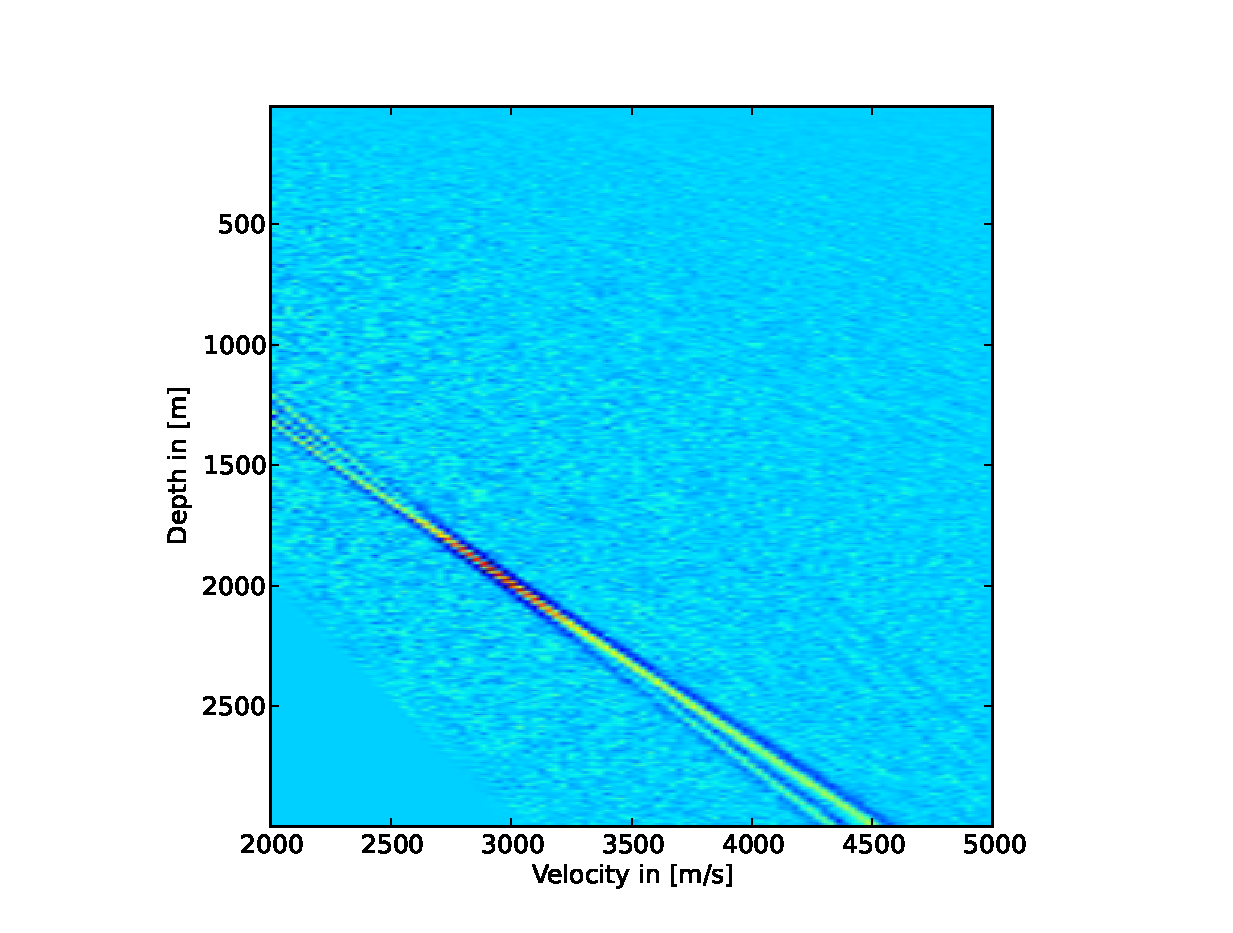
\includegraphics[width=1\textwidth]{v_analysis}
\caption{Geschwindigkeits- Tiefenanalyse}
\label{v_analysis}
\end{figure}

Damit erhalten wir eine Geschwindigkeit von $v = 2950 \frac{m}{s}$ und eine Reflektortiefe von $z=1970 m$.

Wir können somit den theoretischen Zero-Offset Einsatz im Seismogramm bestimmen:

\begin{equation}
	t = \frac{2z}{v} = \frac{2\cdot 1970m}{2950\frac{m}{s}} \approx 1.336s
\end{equation}

Dieses Ergebnis passt sehr gut zum beobachtbaren Einsatz im Seismogramm.


\clearpage
\subsubsection*{d. - Migrierte Sektion}

\begin{verbatim}
>>> k.full_migration(data)
\end{verbatim}

\begin{figure}[htb]
\centering
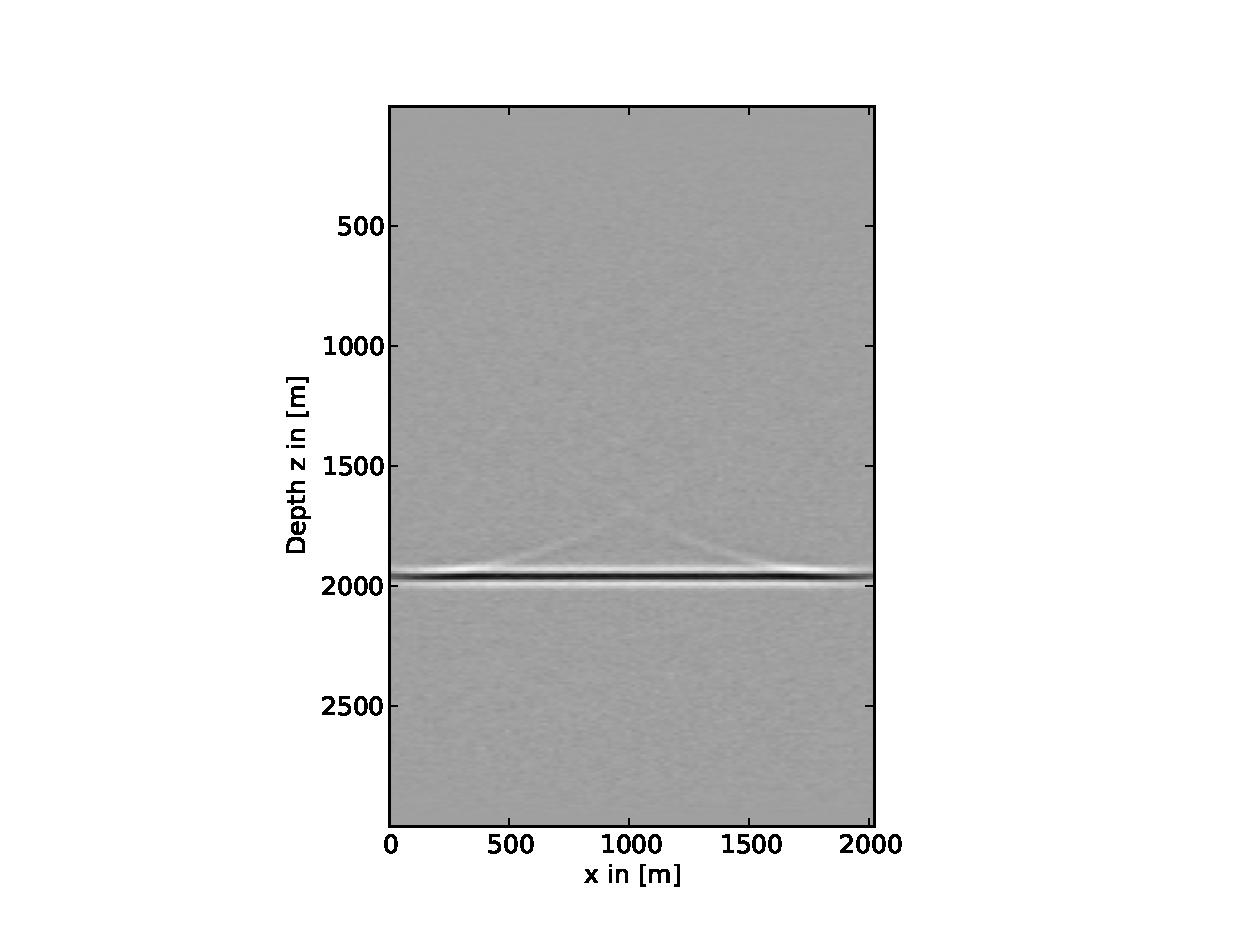
\includegraphics[width=1\textwidth]{full_migration}
\caption{Migrierte Sektion mit $v = 2950\frac{m}{s}$}
\label{full_migration}
\end{figure}

In der migrierten Sektion ist der Reflektor in einer Tiefe von 1970 Metern abgebildet.

Da es sich um eine Linienquelle handelt, lässt sich nicht erkennen, ob Diffraktionen durch die Migration kollabieren. 

Von den Rändern ausgehend sind Artefakte zu erkennen, die durch das abrupte Ende der Spuren zustande kommen.

\clearpage
\subsubsection*{e. - Amplitudenverläufe}

\begin{verbatim}
>>> result = k.full_migration(data)
>>> k.check_amplitudes(result)
\end{verbatim}

\begin{figure}[htb]
\centering
\includegraphics[width=1\textwidth]{amplitudes}
\caption{Maximalamplitude in Abhängigkeit der Spur}
\label{amplitudes}
\end{figure}

In Abbildung \ref{amplitudes} ist zu erkennen, dass die Amplituden zum Rand hin abnehmen. 
Dies dadurch zu erklären, dass an den Rändern nur entlang der einen Hälfte der Diffraktionshyperbel entlang summiert wird. Auf der anderen Seite befinden sich keine Daten mehr.

Interessant sind die Maxima, die auftreten bevor die Amplitude abfällt. Wir vermuten, dass dieses Verhalten mit den Randartefarkten zusammenhängt.

\subsubsection*{h. - Bewertung}



\subsubsection*{i. - Verbesserungsvorschläge}



\begin{figure}[htb]
\centering
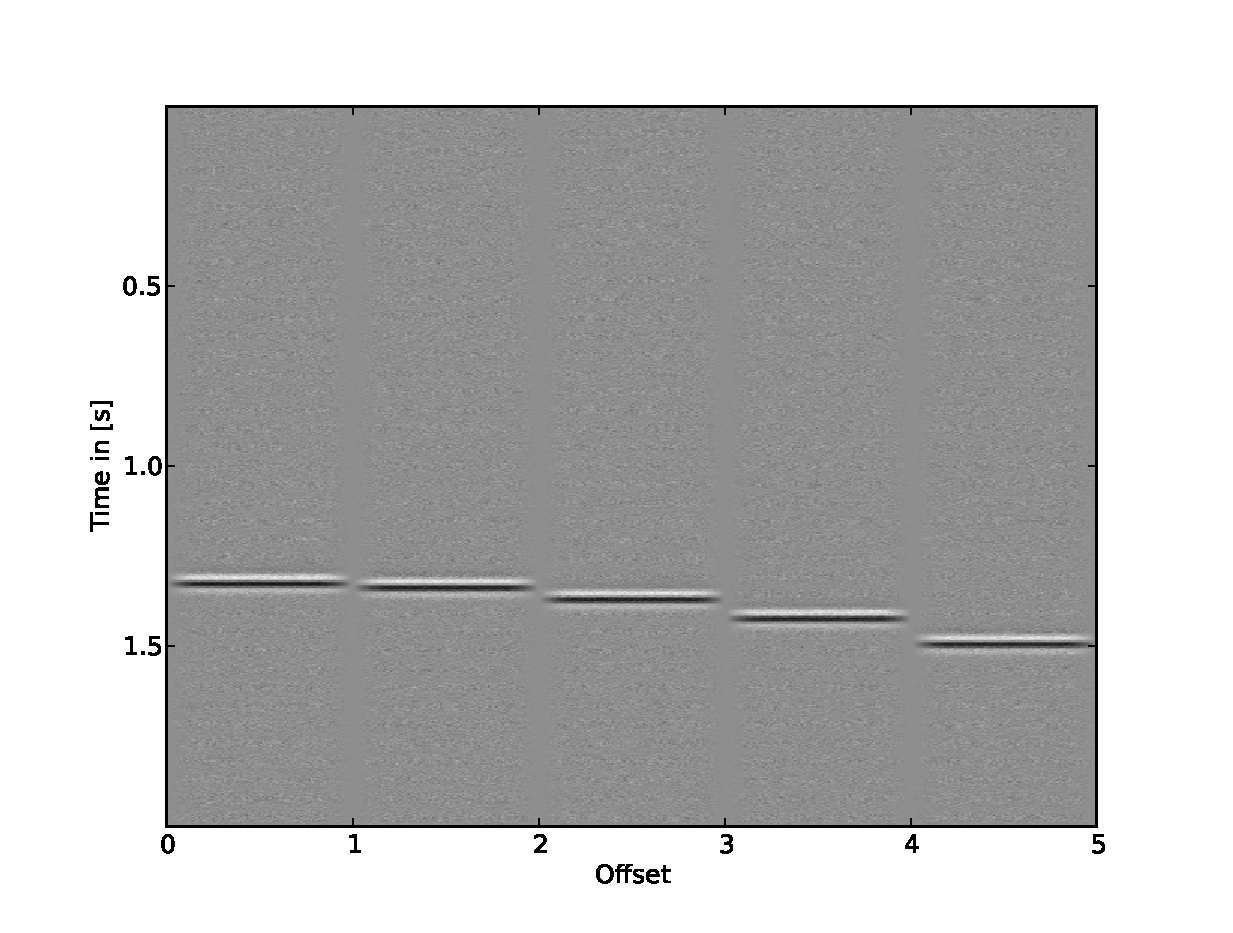
\includegraphics[width=0.7\textwidth]{tapered_data}
\caption{Daten mit einem Taper von 20 Traces}
\label{tapered_data}
\end{figure}

\begin{figure}[htb]
\centering
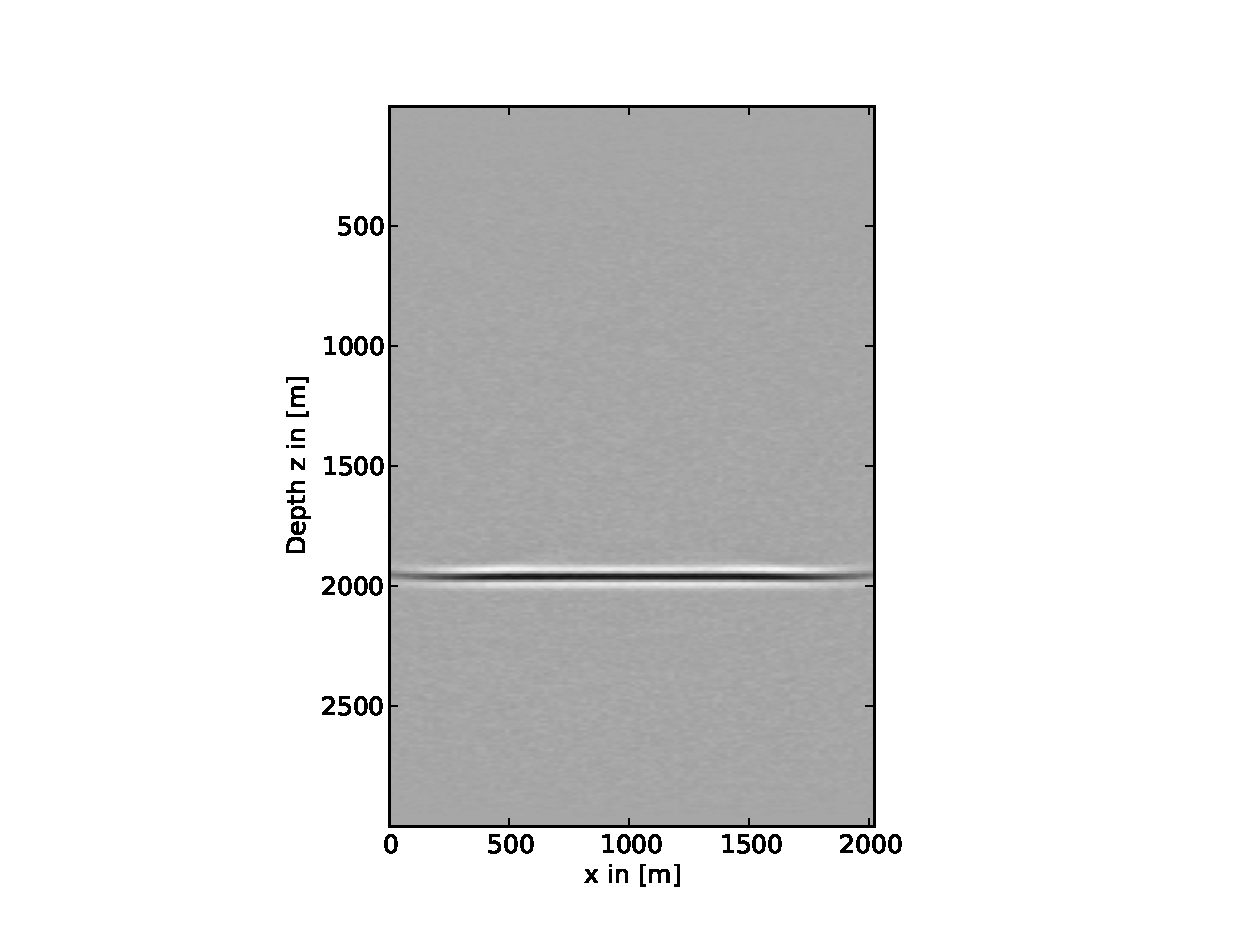
\includegraphics[width=1\textwidth]{tapered_20trc}
\caption{Migrierte Sektion der vorher mit Taper versehenen Daten}
\label{tapered_20trc}
\end{figure}

\clearpage
\subsubsection*{Optimierung des Codes in Cython}

Da Python eine interpretierte Sprache ist und dementsprechend langsam, haben wir den Migrationsalgorithmus noch einmal in \textit{Cython}\footnote{\url{http://cython.org}} implementiert.


\begin{verbatim}
>>> k.benchmark()
Benchmarking python vs cython:
Migrating 10 times with nx= 1
python code:
83.7969629765
cython code:
39.1083641052
\end{verbatim}

Durch die statische Typisierung der Variablen ist der Code etwa doppelt so schnell geworden, ohne dass dadurch die Lesbarkeit beeinträchtigt wurde. 





\end{document}



